\documentclass[11pt]{article}

\usepackage[margin=1.5in]{geometry}
\usepackage{lecnotes}
% \usepackage{mpass}
% \lstset{style=verb,language=mpass}
% logic macros, to be filled from
% lmacros-f21.tex (15-814, F21) and lmacros-f16 (15816, F16)

\newcommand{\ddd}{\raisebox{0.2em}[1.1em]{$\vdots$}}
\newcommand{\vctr}[1]{\begin{array}[c]{c}#1\end{array}}
\newcommand{\CC}{\mathcal{C}}
\newcommand{\DD}{\mathcal{D}}
\newcommand{\EE}{\mathcal{E}}
\newcommand{\FF}{\mathcal{F}}

\newcommand{\ms}[1]{\mathsf{#1}}
\newcommand{\mi}[1]{\mathit{#1}}
\newcommand{\mb}[1]{\mathbf{#1}}
\newcommand{\mt}[1]{\mathtt{#1}}
\newcommand{\ums}[1]{\underline{\ms{#1}}}
\newcommand{\oms}[1]{\overline{\ms{#1}}}
\newcommand{\mc}[1]{\mathcal{#1}}

\newcommand{\uscore}{\mbox{\tt\char`\_}}
\newcommand{\arrow}{\mathbin{\rightarrow}}

\newcommand{\semi}{\mathrel{;}}

% from stmaryrd
\newcommand{\lbb}{\llbracket}
\newcommand{\rbb}{\rrbracket}

% evaluation
\newcommand{\eval}{\ms{eval}}
\newcommand{\evalz}{\ms{eval}_{\mathbb{Z}}}
\newcommand{\evalb}{\ms{eval}_{\mathbb{B}}}

% authorization logic
\newcommand{\says}{\mathrel{\mb{says}}}
\newcommand{\aff}{\mathrel{\mb{aff}}}
\newcommand{\llet}[3]{\mb{let}\; #1 = #2\; \mb{in}\; #3}
\newcommand{\alet}[4]{\mb{let}\; \{#1\}_{#2} = #3\; \mb{in}\; #4}

% \newcommand{\rep}[1]{{}^\ulcorner\! #1{}^\urcorner}

\newcommand{\new}[1]{{\color{blue}#1}}





\newcommand{\course}{15-316: Software Foundations of Security \& Privacy}
\newcommand{\lecturer}{Matt Fredrikson}
\newcommand{\lecdate}{February 5, 2026}
\newcommand{\lecnum}{8}
\newcommand{\lectitle}{Symbolic Evaluation}
\newcommand{\courseurl}{https://15316-cmu.github.io/2024/}

\begin{document}

\maketitle

\section{Introduction}

In the last lecture we introduced the \emph{weakest liberal precondition} which
can be calculated algorithmically from a program as long as loop invariants are
provided by the programmer.  We can then prove $P \arrow [\alpha]Q$ by
delegating $P \arrow \ms{wlp}\; \alpha\; Q$ to a theorem prover for arithmetic,
as long as $P$, $Q$, and any formulas in $\alpha$ are formulas of pure
arithmetic.  The algorithm was based on the \emph{axioms} for dynamic logic we
developed and proved semantically sound.  Variations of this algorithm are used
by systems for program verification such as \href{https://www.why3.org/}{Why3} or
\href{https://dafny.org/}{Dafny}.  In this course we are mostly interested in
verifying safety, which benefits from the same techniques.  Furthermore,
functional verification and safety are often inseparably intertwined.

There is a counterpart to the weakest precondition, namely the \emph{strongest
  postcondition}.  This can also be represented in dynamic logic
\citep{Streett82iandc,Platzer04misc}; you can find a summary in
\href{https://www.cs.cmu.edu/~15414/s22/lectures/11-post.pdf}{Lecture 11} of
15-414 \emph{Bug Catching: Automated Program Verification}.  Here, we approach
it slightly differently, instead devising an algorithm for proving safety by
traversing the program in the order of evaluation.  This is just the opposite of
the weakest precondition which proceeds through the program in reverse order.
This time, instead of using the axioms, we take our inspiration from the rules
of the sequent calculus.  This results in \emph{symbolic evaluation}, and actual
program execution can be seen as a special case.  It is often packaged in the
form of \emph{bounded model checking} \citep{Biere03aic} and available in tools
such as \href{https://www.cprover.org/cbmc/}{CMBC}.

As we will see, there are advantages and disadvantages to both approaches, which
is why both have applications in industry.

\section{Analysis in Evaluation Order}

At the outset, we make the same restriction as in the last lecture: in
$P \arrow [\alpha]Q$, both $P$ and $Q$ are pure, and all formulas occurring in
$\alpha$ are also pure.  Unfortunately, if we want to analyze the program in the
order it is evaluated, this is not quite sufficient.  Consider (for now)
the axiom for sequential composition of programs:
\[
  [\alpha \semi \beta]Q \leftrightarrow [\alpha]([\beta]Q)
\]
Even if we start with a pure postcondition $Q$, on the right-hand side where we
focus on $\alpha$, the postcondition is suddenly $[\beta]Q$.  When you think
about it, this makes sense: if we execute a command in a program, we somehow
have to remember what else needs to be done.  It turns out that the programs
that remain to be executed form a \emph{stack}.  We write $S$ for such formulas
and conjecture that they are sufficient to specify symbolic evaluation.
(Turns out we are right.)
\[
  \begin{array}{lcll}
    \mbox{Stacks} & S & ::= & Q \mid [\alpha]S
  \end{array}
\]
Revisiting the axiom using stacks:
\[
  [\alpha \semi \beta]S \leftrightarrow [\alpha]([\beta]S)
\]
This is now well-formed, because if $S$ is a stack on the left-hand side, the
$[\beta]S$ is a stack on the right-hand side.  We'll have to keep an eye on it,
though.

Next, we consider a specification $P \arrow [\alpha]S$ in the sequent
calculus.  We start the derivation:
\begin{rules}
  \infer[{\arrow}R]
  {\cdot \vdash P \arrow [\alpha]S}
  {P \vdash [\alpha]S}
\end{rules}
It looks like the succedent consists of a single formula $[\alpha]S$, while the
antecedent is also a single (pure) formula $P$.  In order to handle
conditionals, we need to generalize the antecedent.  Consider
\begin{rules}
  \infer[{[\mb{if}]R}]
  {P \vdash [\mb{if}\; P'\; \mb{then}\; \alpha\; \mb{else}\; \beta]S}
  {P, P' \vdash [\alpha]S
    & P, \lnot P' \vdash [\beta]S}
\end{rules}
We see that we accumulate information in the antecedents, so we generalize from
a single formula to a collection $\Gamma$ consisting entirely of pure formulas.

In summary, we will try to define procedure for proving sequents of
the form
\[
  \underbrace{\Gamma}_{\mbox{all pure}} \vdash \underbrace{S}_{\mbox{stack}}
\]

\section{Inference Rules Defining Algorithms}

We already saw one instance where a collection of inference rules described an
algorithm: the sequent rules for propositional calculus in
\href{\courseurl/lectures/02-prop.pdf}{Lecture 2}.  The algorithm
was as follows:
\begin{enumerate}
\item Starting from the sequent we are trying to prove, we arbitrarily use rules
  bottom-up.  Since all rules are invertible (we preserve validity) and
  reductive (we make progress), this is a sound and complete strategy.
\item When we arrive at sequents with only propositional variables we have
  two cases:
  \begin{enumerate}
  \item If antecedents and succedents share a variable $p$, we use the
    identity rule and this subgoal has been proved successfully.
  \item If they are disjoint, we can construct a countermodel (contradicting
    validity) by making all antecedents true and all succedents false.
  \end{enumerate}
\end{enumerate}

We now want to use a similar strategy to construct a derivation of
$\Gamma \vdash S$, under the restrictions motivated in the previous section.  It
will look roughly as follows.
\begin{enumerate}
\item If $S$ is a pure formula $Q$, we call an oracle to prove the
  purely arithmetic sequent.
\item Otherwise, $S = [\alpha]S'$ for some $S'$.  We use the appropriate rule
  for decomposing the program $\alpha$.  Each premise becomes a subgoal.
\end{enumerate}
The rules for $[\alpha]S'$ are \emph{reductive} in the sense that they only
contain constituent programs of $\alpha$ in their premises.  Therefore the
procedure will terminate if each application of the arithmetic oracle
terminates.

For completeness we also need invertibility.  As usual, this holds except for
loops.  However, if we require the programmer to specify loop invariants then a
form of completeness does hold.  We then say that the algorithm is
\emph{complete relative to an oracle for arithmetic}.

Because the form of sequents are restricted compared to the general case of
dynamic logic, we introduce a new notation:
\[
  \Gamma \Vdash S
\]
We will ascertain the property that $\Gamma \Vdash S$ if and only if
$\Gamma \vdash S$, which guarantees the soundness and (relative) completeness of
our algorithm.

\section{Rules for Symbolic Evaluation}

The first is a general (and straightforward) rule: when the succedent is pure,
we call the oracle.  We express this as a sequent consisting entirely of pure
formulas.
\begin{rules}
  \infer[\ms{arith}]
  {\Gamma \Vdash Q}
  {\Gamma \vdash Q & \mbox{$Q$ pure}}
\end{rules}
Like several other rules, the rule for composition is just a restriction of the
rule of the ordinary sequent calculus.
\begin{rules}
  \infer[{[\semi]R}]
  {\Gamma \Vdash [\alpha \semi \beta]S}
  {\Gamma \Vdash [\alpha]([\beta]S)}
\end{rules}
Similarly, assignment remains the same.
\begin{rules}
  \infer[{[{:=}]R^{x'}}]
  {\Gamma \Vdash [x := e]S(x)}
  {\Gamma, x' = e \Vdash S(x') & \mbox{$x'$ fresh}}
\end{rules}
Unlike the situation for the calculation of weakest preconditions, the stack
$S(x)$ may contain programs.  We therefore can only substitute $S(e)$ in some
special cases---generally, we need to make a new assumption and generate a fresh
instance of $x$.

Even for conditionals, not much changes.
\begin{rules}
  \infer[{[\mb{if}]R}]
  {\Gamma \Vdash [\mb{if}\; P\; \mb{then}\; \alpha \;\mb{else}\; \beta]S}
  {\Gamma, P \Vdash [\alpha]S
    & \Gamma, \lnot P \Vdash [\beta]S}
\end{rules}
We can notice something interesting here: we accumulate more information in the
antecedents as we proceed with the (symbolic) evaluation.  This is not the case
when calculating the weakest precondition (or at least not in a straightforward
manner).

Let's consider an example with conditionals:
\[
  \begin{array}{lcl}
    \alpha_1 & = & (\mb{if} \; x \geq 0\; \mb{then}\; y := x\; \mb{else}\; y := -x) \\
    \alpha_2 & = & (\mb{if}\; x \geq 0\; \mb{then}\; z := -x\; \mb{else}\; z := x)\\
    \alpha & = & (\alpha_1 \semi \alpha_2)
  \end{array}
\]
We claim that after this program terminates we have $y + z = 0$.

Let's see how this works out with symbolic evaluation.
\begin{rules}
  \infer[{[\semi]R}]
  {\cdot \Vdash [\alpha_1 \semi \alpha_2]\, (y + z = 0)}
  {\infer[{[\mb{if}]R}]
    {\cdot \Vdash [\alpha_1]([\alpha_2]\, (y + z = 0))}
    {\infer[{[:=]}R]
      {x \geq 0 \Vdash [y := x]([\alpha_2]\, (y + z = 0))}
      {\deduce[(1)]{x \geq 0, y' = x \Vdash [\alpha_2]\, (y' + z = 0)}{}}
      & \deduce[(2)]{\lnot (x \geq 0) \Vdash [y := -x]([\alpha_2]\, (y + z = 0))}{}}}
\end{rules}
Proceeding to $(1)$, we have to apply the rule for conditionals again.
\begin{small}
\begin{rules}
  \hspace*{-3em}
  \infer[{[\mb{if}]R}]
  {x \geq 0, y' = x \Vdash [\alpha_2]\, (y' + z = 0)}
  {\infer[{[:=]R}]
    {x \geq 0, y' = x, x \geq 0 \Vdash [z := -x]\, (y' + z = 0)}
    {\infer[\ms{arith}]
      {x \geq 0, y' = x, x \geq 0, z' = -x \Vdash y' + z' = 0}
      {\deduce[\checkmark]{x \geq 0, y' = x, x \geq 0, z' = -x \vdash y' + z' = 0}{}}}
    & \infer[{[:=]R}]
    {x \geq 0, y' = x, \lnot (x \geq 0) \Vdash [z := x]\, (y' + z = 0)}
    {\deduce[?]{x \geq 0, y' = x, \lnot (x \geq 0), z' = x \Vdash y' + z' = 0}{}}}
\end{rules}
\end{small}

\noindent In the first branch, everything goes according to play.  But in the
second branch, we can read off something like $y' + z' = 2x$ but this is not
equal to $0$!  Fortunately, we can still prove the sequent because the
assumptions $x \geq 0$ and $\lnot (x \geq 0)$ are contradictory.

In fact, we could have stopped just before, when the succedent still contained a
program because the antecedents are already contradictory!  The following rule
allows us to do this in general: we can stop our proof construction as soon as
the antecedents become inconsistent.
\begin{rules}
  \infer[\ms{infeasible}]
  {\Gamma \Vdash S}
  {\Gamma \vdash \bot}
\end{rules}
Since the premise is a pure arithmetic sequent, we directly appeal to the
oracle.  The savings of this rule can be considerable, because the stack $S$
could contain a complex program.  We will return to this in \autoref{sec:paths}
after completing our remaining rules.

We skip the subgoal $(2)$ since it can be proved in a symmetric manner.

\section{Assertions, Tests and Loops}

Assertions and tests are entirely straightforward, since we just
repurpose the ordinary sequent rules.
\begin{rules}
  \infer[{[\mb{assert}]R}]
  {\Gamma \Vdash [\mb{assert}\; P]S}
  {\Gamma \vdash P & \Gamma \Vdash S}
  \hspace{3em}
  \infer[{[\mb{test}]R}]
  {\Gamma \Vdash [\mb{test}\; P]S}
  {\Gamma, P \Vdash S}
\end{rules}
Just note that our assumptions about purity and the stack structure of the
succedents are satisfied.  Also, the first premise immediately appeals to the
oracle since $P$ must be pure.

For loops with invariants, again we mimic the ordinary sequent rule.
\begin{rules}
  \infer[{[\mb{while}]R}]
  {\Gamma \Vdash [\mb{while}_J\; P\; \alpha]S}
  {\Gamma \vdash J
    & J, P \Vdash [\alpha]J
    & J, \lnot P \Vdash S}
\end{rules}
The first premise is pure, but the other two are not by contain stack formulas,
so we remain within the algorithmic rules ($\Vdash$).

An interesting point here is the symbolic evaluation in the presence of loop
invariants is actually \textbf{not} a special case of evaluation: we analyze the
loop body only once, rather than possibly many times as we do when a program is
executed.  This, and the fact that we often won't have loop invariants, leads to
the idea of \emph{bounded symbolic evaluation} or \emph{bounded model checking}.

\section{Control Flow Graphs}
\label{sec:paths}

A pictorial representation of imperative programs, in particular for thinking
about program analysis, are \emph{control flow graphs}.  Since they are also
suitable for low level programs (for example, in assembly language), they are
particularly common in compiler design.

For our purposes, we use an especially simple form.  Small circles denote points
in the program, and arrows indicate possible transitions from one point in the
program to the next.  On the side of the arrow we indicate the \emph{information
  gained} for symbolic evaluation along this particular transition.  For
example, for a conditional
$\mb{if}\; P\; \mb{then}\; \alpha\; \mb{else}\; \beta$ we would draw

\[
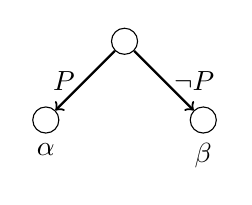
\begin{tikzpicture}
  \node[circle,draw] (a) at (1,2) {};
  \node[circle,draw] (b) at (0,1) [label={below:$\alpha$}] {};
  \node[circle,draw] (c) at (2,1) [label={below:$\beta$}] {};
  \draw[->,thick] (a) -- (b) node[midway,left] {$P$};
  \draw[->,thick] (a) -- (c) node[midway,right] {$\lnot P$};
\end{tikzpicture}
\]

A precondition $P$ is drawn as a label on the incoming edge to the
root.  Starting our example,
\[
  \begin{array}{lcl}
    \alpha_1 & = & (\mb{if} \; x \geq 0\; \mb{then}\; y := x\; \mb{else}\; y := -x) \\
    \alpha_2 & = & (\mb{if}\; x \geq 0\; \mb{then}\; z := -x\; \mb{else}\; z := x)\\
    \alpha & = & (\alpha_1 \semi \alpha_2)
  \end{array}
\]
The precondition is $\top$ and then we have a conditional with two branches.
They come back together before $\alpha_2$. 
\[
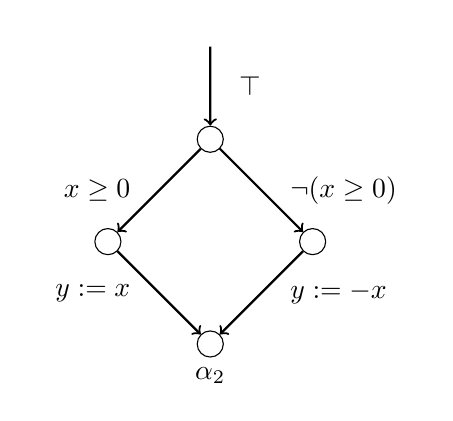
\begin{tikzpicture}[scale=1.3]
  \node (root) at (1,3) {};
  \node[circle,draw] (a) at (1,2) {}; 
  \draw[->,thick] (root) -- (a) node[midway,right,inner sep=1em] {$\top$};
  \node[circle,draw] (b) at (0,1) {};
  \draw[->,thick] (a) -- (b) node[midway,left,inner sep=1em] {$x \geq 0$}; 
  \node[circle,draw] (c) at (2,1) {};
  \draw[->,thick] (a) -- (c) node[midway,right,inner sep=1em] {$\lnot (x \geq 0)$}; 
  \node[circle,draw] (d) at (1,0) [label={below:$\alpha_2$}] {};
  \draw[->,thick] (b) -- (d) node[midway,left,inner sep=1em] {$y := x$}; 
  \draw[->,thick] (c) -- (d) node[midway,right,inner sep=1em] {$y := -x$}; 
\end{tikzpicture}
\]
For an assignment, we just label the arrow with the assignment, although the
``information gained'' will be an equality on a renamed variable.  The program
$\alpha_2$ is represented by a similar graph, starting at the bottom node.
\[
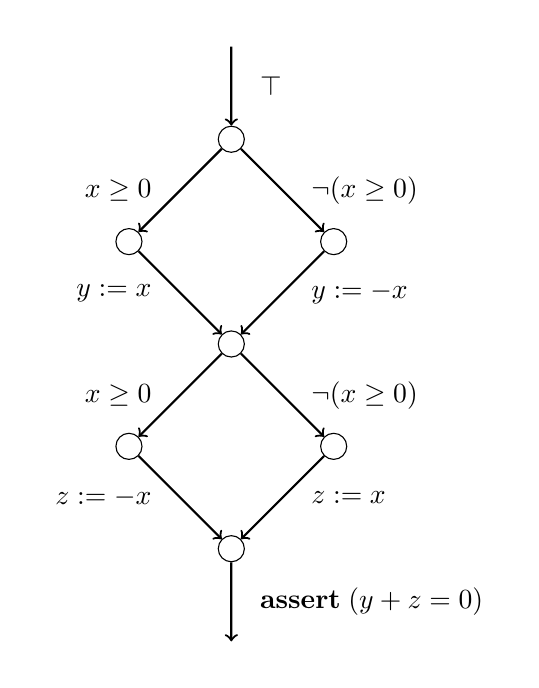
\begin{tikzpicture}[scale=1.3]
  \node (root) at (1,3) {};
  \node[circle,draw] (a) at (1,2) {}; 
  \draw[->,thick] (root) -- (a) node[midway,right,inner sep=1em] {$\top$}; 
  \node[circle,draw] (b) at (0,1) {}; 
  \draw[->,thick] (a) -- (b) node[midway,left,inner sep=1em] {$x \geq 0$}; 
  \node[circle,draw] (c) at (2,1) {};
  \draw[->,thick] (a) -- (c) node[midway,right,inner sep=1em] {$\lnot (x \geq 0)$}; 
  \node[circle,draw] (d) at (1,0) {};
  \draw[->,thick] (b) -- (d) node[midway,left,inner sep=1em] {$y := x$}; 
  \draw[->,thick] (c) -- (d) node[midway,right,inner sep=1em] {$y := -x$}; 
  %
  \node[circle,draw] (e) at (0,-1) {};
  \draw[->,thick] (d) -- (e) node[midway,left,inner sep=1em] {$x \geq 0$}; 
  \node[circle,draw] (f) at (2,-1) {}; 
  \draw[->,thick] (d) -- (f) node[midway,right,inner sep=1em] {$\lnot (x \geq 0)$}; 
  \node[circle,draw] (h) at (1,-2) {};
  \draw[->,thick] (e) -- (h) node[midway,left,inner sep=1em] {$z := -x$}; 
  \draw[->,thick] (f) -- (h) node[midway,right,inner sep=1em] {$z := x$}; 
  %
  \node (i) at (1,-3) {};
  \draw[->,thick] (h) -- (i) node[midway,right,inner sep=1em] {$\mb{assert}\; (y + z = 0)$};
\end{tikzpicture}
\]
A \emph{path} through this program just follows the arrows from the root down to
the final node.  A priori, each path represents a potential execution of the
program.  It is easy to see that the number of paths through a control flow
graph could be exponential in its size.

Viewed in terms of the sequent calculus, each path represents a branch in the
proof tree, looking upwards.  A \emph{path formula} is the conjunction of
the information gained along a path (which includes some renaming for variable
assignments).  The output $\mb{assert}$ represents the postcondition in the
succedent of the sequent.  For example, going left both times gives us the
sequent
\[
  x \geq 0, y' = x, x \geq 0, z' = -x \vdash y' + z' = 0
\]
If we first go left and then right we can stop even before the assignment
because the path reads
\[
  x \geq 0, y' = x, \lnot (x \geq 0) \vdash \ldots
\]
which is \emph{infeasible}.  In this example, there are only two feasible
paths, and the postcondition holds for both of them.

\section{Bounded Symbolic Evaluation}

When there are no loop invariants (or maybe they aren't sufficient for our
purposes), symbolic evaluation offers another option.  We can \emph{unroll each
  loop} to a certain specified depth.  The depth is necessary in many cases in
order to avoid nontermination of the algorithm.  Recall the axiom
\[
  [\mb{while}\; P\; \alpha]Q \leftrightarrow (P \arrow [\alpha]([\mb{while}\; P\; \alpha]Q))
  \land (\lnot P \arrow Q)
\]
and the corresponding rule:
\begin{rules}
  \infer[\ms{unfold}]
  {\Gamma \vdash [\mb{while}\; P\; \alpha]Q, \Delta}
  {\Gamma, P \vdash [\alpha]([\mb{while}\; P\; \alpha]Q), \Delta
    & \Gamma, \lnot P \vdash Q, \Delta}
\end{rules}
In this rule we don't lose $\Gamma$ and $\Delta$ because we go around the loop
exactly 1 or 0 times.  The $\ms{unfold}$ rule is not reductive.  In order to
represent \emph{bounded} evaluation we annotate the $\mb{while}$ with $n$, a
constant natural number not accessible to the programmer.  Instead, it would
usually be a parameter to an invocation of a bounded model checker.  Then we
have two rules: one when we are still allowed to unroll the loop, and one when
we have reached the bound.
\begin{rules}
  \infer[\ms{unfold}^{n+1}]
  {\Gamma \Vdash [\mb{while}^{n+1}\; P\; \alpha]S}
  {\Gamma, P \Vdash [\alpha]([\mb{while}^n\; P\; \alpha]S)
    & \Gamma, \lnot P \Vdash S}
  \hspace{2em}
  \infer[\ms{unfold}^0]
  {\Gamma \Vdash [\mb{while}^0\; P\; \alpha]S}
  {\Gamma \Vdash S}
\end{rules}
The rules are now reductive in the sense that the pair $(\alpha, n)$ decreases:
either $n$ becomes smaller and the program remains the same, or $n$ has reached
$0$ and then the program becomes smaller.  This is called a \emph{lexicographic
  ordering} because two pairs are compared first in their first component and
then in their second if the first are equal.  This is like the ordering of words
in a dictionary.

These rules have several problems.  A critical one is that we may not be
guaranteed that the loop without the depth annotation actually satisfies the
postcondition.  If we can prove all subgoals we know at least that there isn't
an obvious problem that would arise by limited execution.  And if there is a
bug, we might still find it by generating a subgoal that is not provable.
Therefore we might say that bounded symbolic evaluation is for \emph{bug
  finding}, but generally not for full verification.

In some circumstances, even bounded checking could amount to full verification.
That's when the paths around the loop become infeasible before the bound is
reached.  Sequent derivations are large and awkward to show, so we use a control
flow graph instead for the (by now familiar) program
\[
  0 \leq x \leq 3 \arrow [\mb{while}\; (x > 1); x := x-2]\, (0 \leq x \leq 1)
\]
with a new precondition.

Because we have a loop, the control flow graph will now have a back edge,
pointing up higher in the graph.
\[
  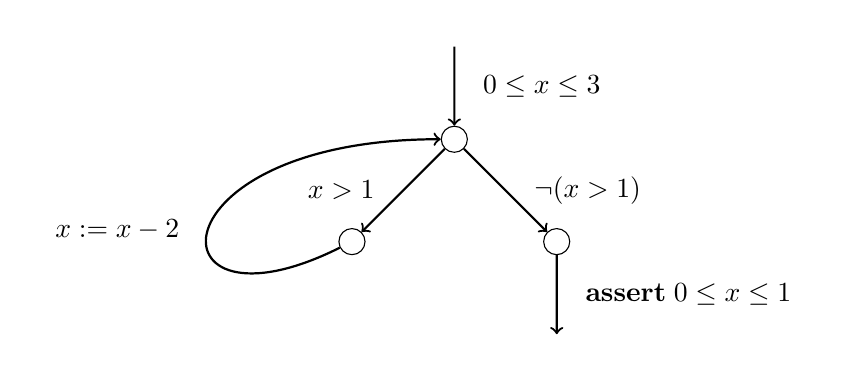
\begin{tikzpicture}[scale=1.3]
    \node (root) at (1,3) {};
    \node[circle,draw] (a) at (1,2) {};
    \draw[->,thick] (root) -- (a) node[midway,right,inner sep=1em] {$0 \leq x \leq 3$};
    \node[circle,draw] (b) at (0,1) {};
    \draw[->,thick] (a) -- (b) node[midway,left,inner sep=1em] {$x > 1$};
    \node[circle,draw] (c) at (2,1) {};
    \draw[->,thick] (a) -- (c) node[midway,right,inner sep=1em] {$\lnot (x > 1)$};
    \draw[->,thick] (b) .. controls (-2,0) and (-2,2) .. (a) node[midway,left,inner sep=1em] {$x := x-2$};
    \node (e) at (2,0) {};
    \draw[->,thick] (c) -- (e) node[midway,right,inner sep=1em] {$\mb{assert}\; 0 \leq x \leq 1$};
  \end{tikzpicture}
\]
We enumerate the sequents along the paths, which are marked with $\ms{R}$ (for
chosing the right alternative, leaving the loop) and $\ms{L}$ for chosing the
left one (proceeding into the loop).
\[
  \begin{array}{lcll}
    \ms{R} & : & 0 \leq x \leq 3, \lnot (x > 1) \vdash 0 \leq x \leq 1 & \mbox{valid!} \\
    \ms{LR} & : & 0 \leq x \leq 3, x > 1, x' = x-2, \lnot (x' > 1) \vdash 0 \leq x' \leq 1 & \mbox{valid!} \\
    \ms{LL} & : & 0 \leq x \leq 3, x > 1, x' = x-2, x' > 1 \vdash \ldots & \mbox{infeasible!}
  \end{array}
\]
The last path doesn't go all the way to the end, because the partial path
$\ms{LL}$ is already contradictory.  The path being infeasible means that the
sequent is valid using the rule $\ms{infeasible}$.  So in this example the
precondition was strong enough that we were able to prove validity with just two
iterations of the loop.

\section{Summary}

We summarize the rules for symbolic evaluation, alternatively with loop
invariants or bounds on loop unrolling, in \autoref{fig:symeval}.  In order to
prove $P \arrow [\alpha]Q$ for pure $P$ and $Q$ (and $\alpha$ only containing
pure conditions), we search bottom-up for a proof of $P \Vdash [\alpha]Q$.  Also
recall the definition of stacks
\[
  \begin{array}{lcll}
    \mbox{Stacks} & S & ::= & Q \mid [\alpha]S
  \end{array}
\]
By the way, we can recover ordinary execution from symbolic evaluation by
proceeding as in bounded evaluation (unrolling the loop), without regard to any
bound.  This only makes sense if our antecedents assign a constant value to each
variable that is used by the program.  In that case, each time we might branch
due to a conditional or loop, one side will immediately be infeasible and we
proceed deterministically.  Of course, evaluation may not terminate.

This is not a particularly clever way to evaluate a program because of the
frequent renaming.  Essentially, the antecedents keep track of the whole history
of the computation, that is, every value that a variable had on the current (and
only) path.  One could improve on that, but there are also more direct ways to
obtain evaluation from the semantic definition of $\omega \lbb\alpha \rbb \nu$.

\begin{figure}[ht]
  \begin{rules}
  \infer[\ms{arith}]
  {\Gamma \Vdash Q}
  {\Gamma \vdash Q & \mbox{$Q$ pure}}
  \hspace{3em}
  \infer[\ms{infeasible}]
  {\Gamma \Vdash S}
  {\Gamma \vdash \bot}
  \\[1em]
  \infer[{[\semi]R}]
  {\Gamma \Vdash [\alpha \semi \beta]S}
  {\Gamma \Vdash [\alpha]([\beta]S)}
  \hspace{3em}
  \infer[{[{:=}]R^{x'}}]
  {\Gamma \Vdash [x := e]S(x)}
  {\Gamma, x' = e \Vdash S(x') & \mbox{$x'$ fresh}}
  \\[1em]
  \infer[{[\mb{if}]R}]
  {\Gamma \Vdash [\mb{if}\; P\; \mb{then}\; \alpha \;\mb{else}\; \beta]S}
  {\Gamma, P \Vdash [\alpha]S
    & \Gamma, \lnot P \Vdash [\beta]S}
  \\[1em]
  \infer[{[\mb{assert}]R}]
  {\Gamma \Vdash [\mb{assert}\; P]S}
  {\Gamma \vdash P & \Gamma \Vdash S}
  \hspace{3em}
  \infer[{[\mb{test}]R}]
  {\Gamma \Vdash [\mb{test}\; P]S}
  {\Gamma, P \Vdash S}
  \\[1em]
  \infer[{[\mb{while}]R}]
  {\Gamma \Vdash [\mb{while}_J\; P\; \alpha]S}
  {\Gamma \vdash J
    & J, P \Vdash [\alpha]J
    & J, \lnot P \Vdash S}
  \\[1em]\hline\\[1ex]
  \infer[\ms{unfold}^{n+1}]
  {\Gamma \Vdash [\mb{while}^{n+1}\; P\; \alpha]S}
  {\Gamma, P \Vdash [\alpha]([\mb{while}^n\; P\; \alpha]S)
    & \Gamma, \lnot P \Vdash S}
  \hspace{2em}
  \infer[\ms{unfold}^0]
  {\Gamma \Vdash [\mb{while}^0\; P\; \alpha]S}
  {\Gamma \Vdash S}
  \end{rules}
  \caption{Symbolic Evaluation}
  \label{fig:symeval}
\end{figure}

\bibliographystyle{plainnat}
\bibliography{bibliography}

\end{document}
